\documentclass[11pt]{article}

\usepackage{float}
\usepackage{hyperref}
\usepackage{graphicx}
% formatting
\usepackage{fullpage}
\usepackage{verbatim}
\usepackage{moreverb}
\usepackage{minted}
\usepackage{amsmath}
\usepackage{parskip}
\let\verbatiminput=\verbatimtabinput
\def\verbatimtabsize{4\relax}

\begin{document}
\title{EE 142 Problem Set 3}

\author{Vighnesh Iyer}
\date{}
\maketitle

\section{T-Lines at Steady State}

\begin{figure}[H]
	\centering 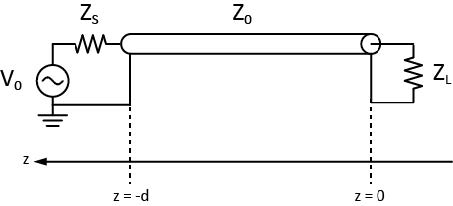
\includegraphics[width=\textwidth-7cm]{images/problem1.jpg}
\end{figure}

Voltage source generates 10 Ghz sine with 10V amplitude.

Tline terminated with $Z_L = 80 - 40j \Omega$, and $Z_0 = 100\Omega$. $\epsilon_{eff} = 4$ and $d = 22.5$ mm.

\begin{enumerate}
	\item Find the reflection coefficient at the load (z = 0) and at the source (z = -d)
	
	At the load:
	
	\begin{align*}
		\rho_L &= \frac{Z_L - Z_0}{Z_L + Z_0} \\
		\rho_L &= -0.0588 - 0.23539j \\
		|\rho_L| &= 0.242
	\end{align*}
	
	At any point on the line, we can derive an effective generalized $\rho(z)$ which represents the ratio of the backwards and forward traveling waves at a given point on the tline.
	
	\begin{align*}
		V(z) &= V_0^+ (e^{-j \beta z} + \rho_L e^{-j \beta z}) \\
		\rho(z) &= \frac{V_0^+ \rho_L e^{j \beta z}}{V_0^+ e^{-j \beta z}} \\
		\rho(z) &= \rho_L e^{2j \beta z}
	\end{align*}
	
	Notice that since $\beta = 2\pi / \lambda$, $\rho(z)$ repeats every $\lambda / 2$ traversed along the tline back to the generator. We can find $c_p$ and $\lambda$ for this tline and frequency.
	
	\begin{align*}
		c_p &= \frac{c_0}{\sqrt{\epsilon_{eff}}} \approx 1.5e8 \text{ m/s} \\
		\lambda &= \frac{c_p}{f} = 0.015 \text{ m} \\
		d / \lambda = 1.5 = 3 \cdot \frac{1}{2} \lambda \\
	\end{align*}
	
	So, $\rho(z)$ at $z = -d$ is $rho_L = 0.242$.
	
	\item Find the input impedance at the source (z = -d) and at z = 18.75mm.
	
	The general form is:
	
	\begin{align*}
		Z_{in}(-l) &= Z_0 \frac{Z_L + j Z_0 \tan(\beta l)}{Z_0 + j Z_L \tan(\beta l)} \\
		\beta &= \frac{2 \pi}{\lambda} = 418.879 \\
		Z_{in}(0) &= Z_L = 100 \Omega \\
		Z_{in}(-18.75 \text{ mm}) &= Z_{in}(\lambda + \lambda / 4) = \frac{Z_0^2}{Z_L} = 100 + 50j \\
	\end{align*}
	
	\item Plot the magnitude of the voltage along the line. Find voltage maximum, minimum, and SWR.
	
	We assume that $Z_S$ = $Z_0$:
	
	\begin{align*}
		SWR &= \frac{V_{max}}{V_{min}} = \frac{1 + |\rho_L|}{1 - |\rho_L|} \\
		SWR &= 1.64 \\
		V^+ &= \frac{Z_0}{Z_0 + Z_S} = 5 \text{ V} \\
		V_{max} &= |V^+| (1 + |\rho_L|) = 6.2 \text{ V} \\
		V_{min} &= |V^+| (1 - |\rho_L|) = 3.8 \text{ V} 
	\end{align*}
	
	Plot of voltage magnitude along line:
	\begin{figure}[H]
		\centering 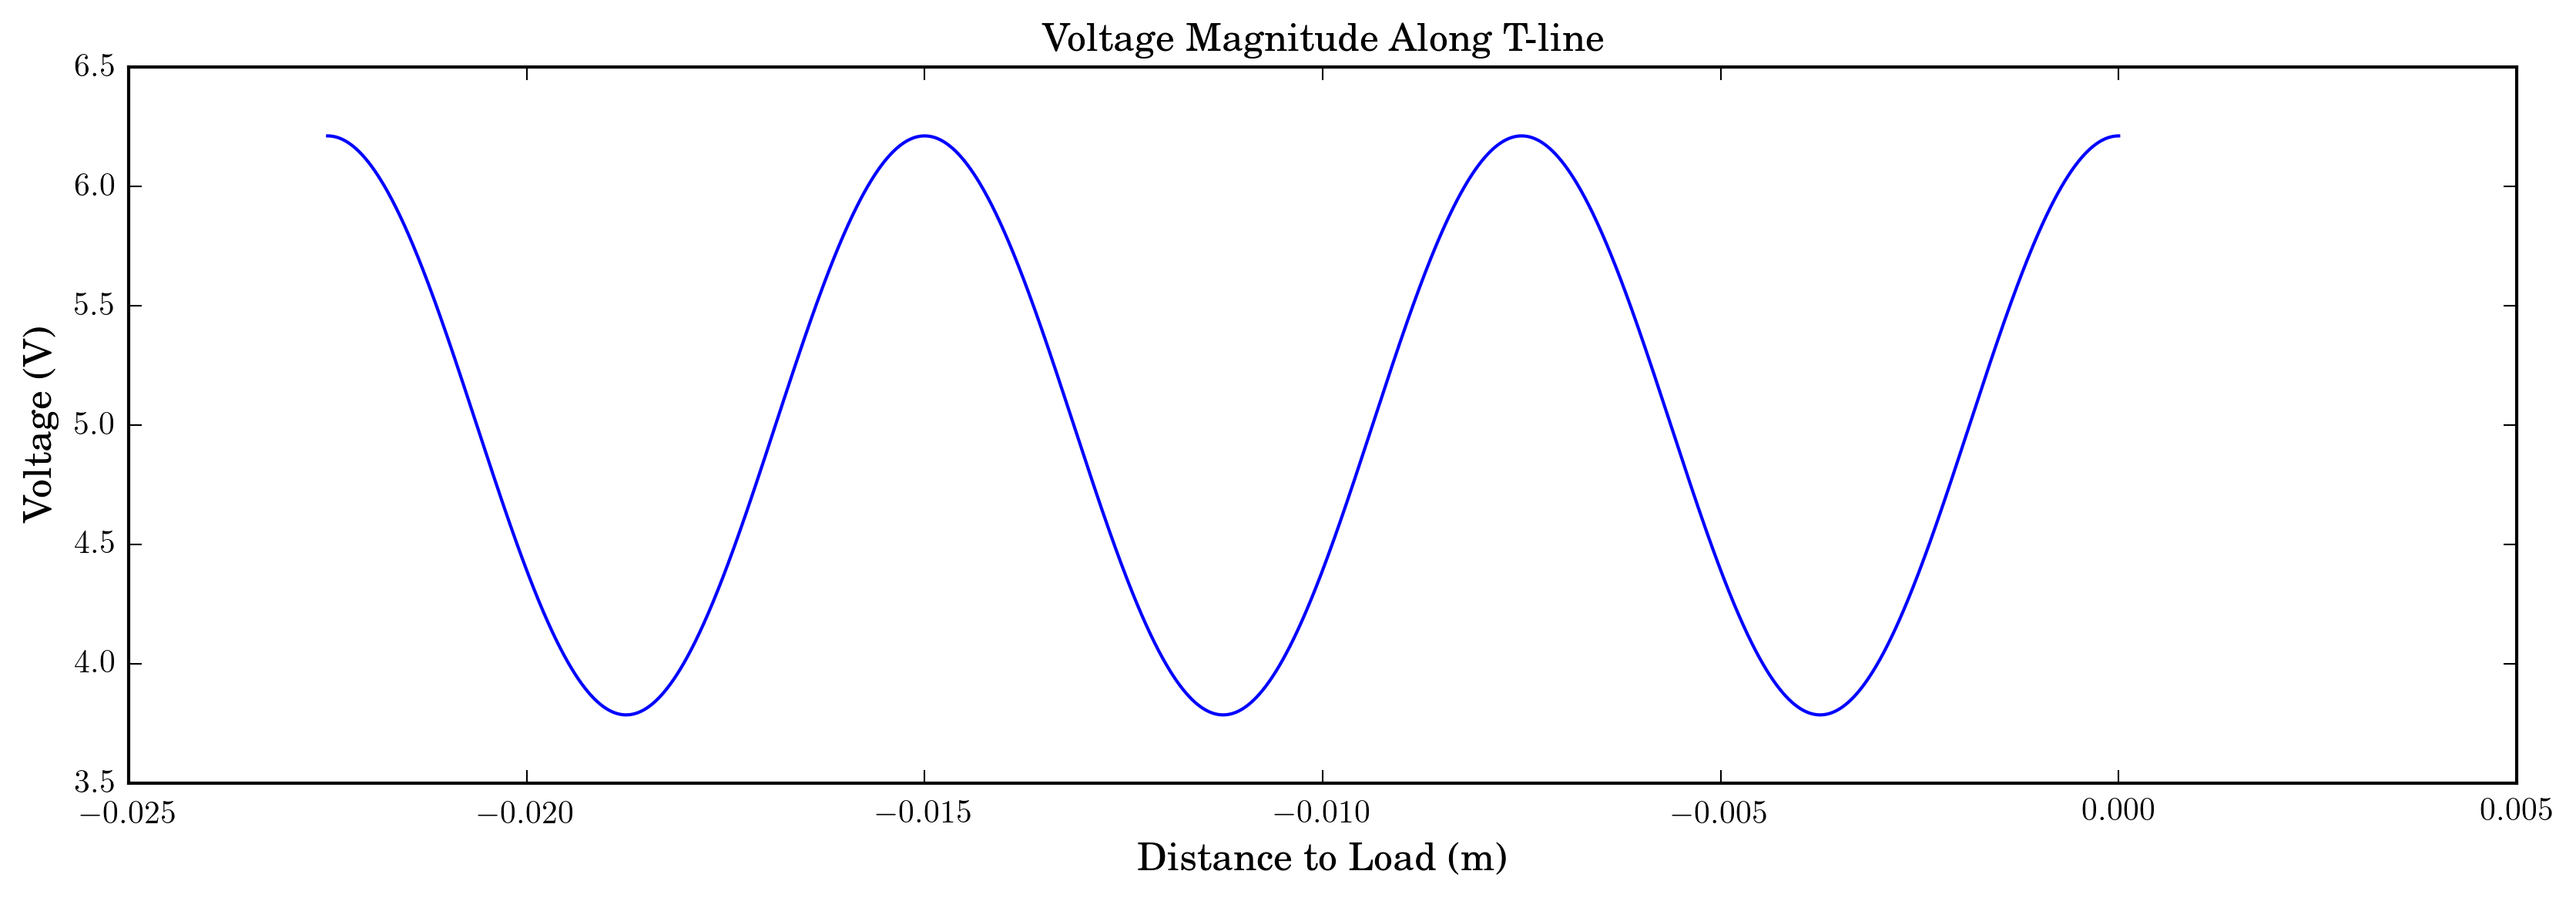
\includegraphics[width=\textwidth]{images/problem1.png}
	\end{figure}
\end{enumerate}

\section{T-Line Modeling}
We will derive an equivalent two-port circuit model for a short section of transmission line ($l << \lambda$) including loss.

\begin{enumerate}
	\item For a "pi" equivalent circuit shown below, find the two-port Z matrix.
	\begin{figure}[H]
		\centering 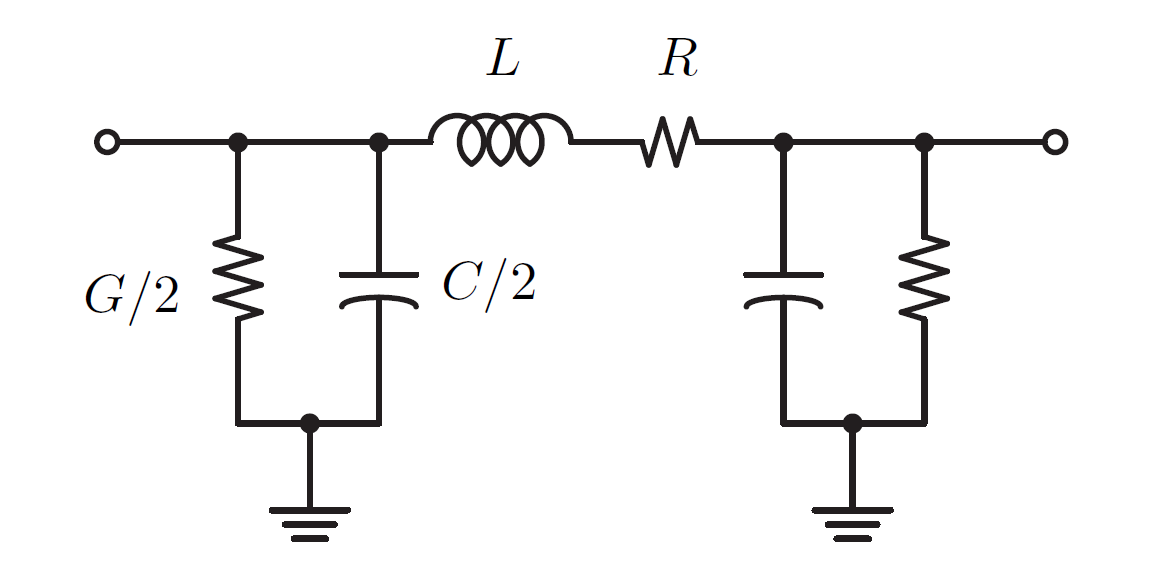
\includegraphics[width=\textwidth-6cm]{images/problem2_pi_network.png}
	\end{figure}
	
\end{enumerate}

\section{Impedance Matching for Maximum Power Delivery}

\begin{enumerate}
	\item What is the maximum power that can be extracted from the source shown below? What is the optimal load impedance for the maximum power delivery to happen?
		\begin{figure}[H]
		\centering 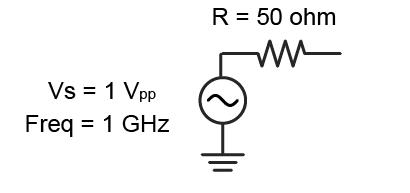
\includegraphics[width=\textwidth-10cm]{images/problem3a.jpg}
	\end{figure}
	
	\begin{align*}
		|I_{s}| &= \frac{|V_s|}{|R_s + R_L|} \\
		I_{s,rms} &= \frac{1}{2} |I_{s}| \\
		V_{L} &= I_{s,rms} R_L \\
		P_{L} &= I_{s,rms} V_L = I_{s,rms}^2 R_L = 1/2 (\frac{V_s}{R_s + R_L})^2 R_L \\
		\frac{\partial P_L}{\partial R_L} &= (\frac{-R_s}{R_L})^2 + 1
	\end{align*}
	
	Setting the denominator of derivative to 0 and solving gives $R_L = \pm R_s \rightarrow R_L = R_s$. Indeed, this minimizes the denominator, and thus maximizes the power delivered to the load.
	
	\begin{align*}
		P_{max} = \frac{V_s^2}{8 R_L} = 2.5 \text{ mW}
	\end{align*}
	
	\item Use this source to drive a $500\Omega$ load ans we directly connect the load to the source, as illustrated by the figure below. What is the power delivered to the $500 \Omega$ load and the load voltage?
	
	\begin{figure}[H]
		\centering 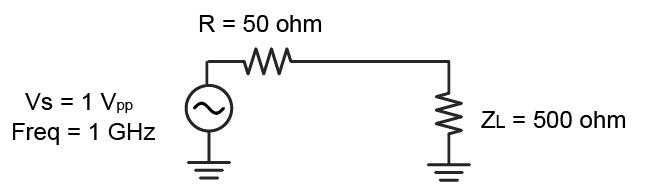
\includegraphics[width=\textwidth-8cm]{images/problem3b.jpg}
	\end{figure}

	\begin{align*}
		P_L = 0.8 \text{ mW} \\
		V_L = I_{s,rms} R_L = 0.45 \text{ V}
	\end{align*}
	
	\item Let's try to achieve impedance matching by putting a quarter-wavelength transmission line between the load and source, as indicated by the below figure. Find the characteristic impedance $Z_0$ that maximizes the power delivered to the load. What are the corresponding power and voltage at the load?
	
	\begin{figure}[H]
		\centering 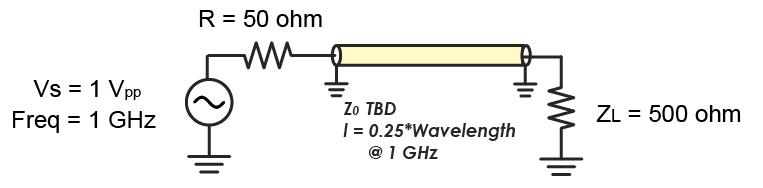
\includegraphics[width=\textwidth-8cm]{images/problem3c.jpg}
	\end{figure}
\end{enumerate}

\end{document}
